\documentclass[11pt]{article}
\usepackage[sc]{mathpazo} %Like Palatino with extensive math support
\usepackage{fullpage}
\usepackage[authoryear,sectionbib,sort]{natbib}
\linespread{1.7}
\usepackage[utf8]{inputenc}

%%%%%%%%%%%%%%%%%%%%%
% LaTeX packages
%%%%%%%%%%%%%%%%%%%%%
% Please be sparing in your use of additional LaTeX packages, and
% upload any required style files to Editorial Manager with the file
% type "LaTeX ancillary files (.sty, .bst)."
\usepackage{amsmath,amssymb}
%\usepackage{graphicx}
%\graphicspath{ {IMAGES/} }

%%%%%%%%%%%%%%%%%%%%%
% Line numbering
%%%%%%%%%%%%%%%%%%%%%
%\usepackage{lineno}
% Please use line numbering with your initial submission and
% subsequent revisions. After acceptance, please comment out 
% the commands \usepackage{lineno}, \linenumbers{} 
% and \modulolinenumbers[3] below.

\title{Warming induced changes to body size stabilize consumer-resource dynamics}

%%%%%%%%%%%%%%%%%%%%%
% Authorship
%%%%%%%%%%%%%%%%%%%%%
% Please remove authorship information while your paper is under review,
% unless you wish to waive your anonymity under double-blind review. 
% Remember to uncomment the information after acceptance.

\author{
Matthew M Osmond$^{1,\ast}$, \\ 
Matthew A Barbour$^{1,2}$, \\
Joey R Bernhardt$^{1}$, \\
Matthew W Pennell$^{1}$, \\
Jennifer M Sunday$^{1}$, \\
Mary I O'Connor$^{1}$ 
}

\date{}

\begin{document}

\maketitle

\noindent{}1. Biodiversity Research Centre and Department of Zoology, University of British Columbia, Canada;

\noindent{}2. Department of Evolutionary Biology and Environmental Studies, University of Zurich, Switzerland;

\noindent{}$\ast$ Corresponding author; e-mail: mmosmond@zoology.ubc.ca.

\bigskip

\textit{Manuscript elements}: Figure~1, table~1, supplementary material (\texttt{Mathematica} file and PDF copy).
\bigskip

\textit{Keywords}: Metabolic scaling theory, predator-prey, plant-herbivore, functional response, mathematical model, temperature-size rule.

\bigskip

\textit{Manuscript type}: Note. 
% Or e-article, note, e-note, natural history miscellany,
% e-natural history miscellany, comment, reply, symposium, or
% countdown to 150.

\bigskip

\noindent{\footnotesize Prepared using the suggested \LaTeX{} 
template for \textit{Am.\ Nat.}}

%\linenumbers{}
%\modulolinenumbers[3]

\newpage{}

%%%%%%%%%%%%%%%%%%%%%%%%%%%%%%%%%%%%%%%%%%%%%%%%
\section*{Abstract}
%%%%%%%%%%%%%%%%%%%%%%%%%%%%%%%%%%%%%%%%%%%%%%%%
Both body size and temperature directly influence consumer-resource dynamics. There is also widespread empirical evidence for the temperature-size rule (TSR), which creates a negative relationship between temperature and body size. However, it is not known how the TSR affects community dynamics. Here we integrate temperature- and size-dependent models to include indirect effects of warming, through changes in body size, to answer the question: How does the TSR affect the predicted response of consumer-resource systems to warming? We find that the TSR is expected to maintain consumer-resource biomass ratios and buffer the community from extinctions under warming. While our results are limited to conditions where organisms are below their thermal optimum, they hold under a range of realistic temperature-size responses and are robust to the type of functional response. 
Our analyses suggest that the widely observed TSR may reduce the impacts of warming on consumer-resource systems.

\newpage{}

%%%%%%%%%%%%%%%%%%%%%%%%%%%%%%%%%%%%%%%%%%%%%%%%
\section*{Introduction}
%%%%%%%%%%%%%%%%%%%%%%%%%%%%%%%%%%%%%%%%%%%%%%%%

% The journal does not have numbered sections in the main portion of
% articles. Please refrain from using section references such as
% section~\ref{section:CountingOwlEggs}, and refer to sections by name
% (e.g. section ``Counting Owl Eggs'').

% Please note that we prefer (\citealt{Xiao2015}) to \citealt{Xiao2015},
% since \citealt{} inserts a comma after "et al."

Consumer-resource interactions are a fundamental aspect of ecological communities.
The strength and stability of these interactions generate patterns in the structure and functioning of ecosystems, dictating the flow of energy between trophic levels. 
Due to the temperature-dependence of metabolism \citep{Gillooly2001}, rates of birth, death, and consumption vary with temperature \citep{Savage2004,Gilbert2014}.
Thus the flow of energy from resource to consumer often changes under warming, and even small changes in temperature that are not necessarily physiologically stressful can affect stability and coexistence, producing predictable effects of warming on simple food webs \citep{Gilbert2014,Vasseur2005,OConnor2011,Rall2010}. 

Warming also causes predictable changes in body size.
For example, adult body size tends to decline with temperature during ontogeny \citep[the temperature-size rule, TSR; reviewed in][]{Atkinson1994} and mean body size often declines towards the equator, both between and within species \citep[Bergmann's rule; reviewed in][]{Blackburn1999}.
Although the mechanism varies (e.g., phenotypic plasticity in the case of the TSR, selection for smaller individuals and species turnover in the case of Bergmann's rule), the pattern is similar and declining body size with warming is considered a universal response to warming \citep{Daufresne2009,Gardner2011}. 
Here we focus on the TSR, where plastic changes in body size occur rapidly relative to population dynamics.

Because body size \citep{Yodzis1992,DeLong2015} and body size ratios \citep{Kalinkat2013} affect demographic rates and hence consumer-resource dynamics, such a systematic pattern of changing body sizes with temperature could alter predictions for how temperature affects stability
and coexistence in consumer-resource systems. 
To formally explore this possibility, we integrated the TSR into a general framework for temperature-dependent consumer-resource interactions to answer the question: 
How does the TSR affect the predicted response of  consumer-resource interaction strength, equilibrium consumer:resource biomass ratios, and community 
stability to warming? 
We then explored the effect of the magnitude of body size-temperature scaling, under both a type-I and type-II functional response, including cases where the scaling differs between consumers and their resources. 
Because body size changes may also affect the overall functional response \citep[e.g., changes from type-II to type- III;][]{Kalinkat2013}, we also explored (in the supplementary material) whether changes in temperature might induce a change in functional response through body size-temperature responses as described by the TSR. 

%%%%%%%%%%%%%%%%%%%%%%%%%%%%%%%%%%%%%%%%%%%%%%%%%%%
\section*{Methods and results}
%%%%%%%%%%%%%%%%%%%%%%%%%%%%%%%%%%%%%%%%%%%%%%%%%%%

%%%%%%%%%%%%%%%%%%%%%%%%%%%
\subsection*{The underlying consumer-resource dynamics}
We begin, like \cite{Gilbert2014}, with a general consumer-resource model
\begin{equation}\label{eq:RM}
\begin{aligned}
\frac{\mathrm{d}R}{\mathrm{d}t} =& r R \left(1 - \frac{R}{K} \right) - f(R) R C\\
\frac{\mathrm{d}C}{\mathrm{d}t} =& e f(R) R C - m C,
\end{aligned}
\end{equation}
which describes the rates of change in total resource $R\in[0,K]$ and consumer $C\geq0$ biomass with time $t$.

In the absence of consumers, $C=0$, the resource grows logistically, with intrinsic growth rate $r\geq0$ and carrying capacity $K>0$.
The intrinsic growth rate describes the rate at which resource biomass increases (per unit biomass) in the absence of consumers when the resource is rare, $R\approx0$.
The carrying capacity is the equilibrium biomass of the resource without consumers.

Resource biomass is consumed by consumers at a rate $f(R) R C$, where $f(R) R\geq0$ is called the functional response.
Of the biomass consumed, the unitless conversion efficiency parameter $e\in[0,1]$ determines the proportion of resource biomass that is directly converted into consumer biomass.
Consumer biomass dies at a constant per unit biomass mortality rate $m\geq0$.

An equilibrium is reached when the two rates of change in Equation \eqref{eq:RM} are zero, and solving the system at this point gives equilibrium resource $\hat{R}$ and consumer $\hat{C}$ biomass.
At the coexistence equilibrium (i.e., where both $\hat{C}$ and $\hat{R}$ $>0$) one can calculate the ratio of consumer to resource biomass, $\hat{C}:\hat{R}$, and also perform a linear stability analysis to derive the dominant (largest in absolute value) eigenvalue, $\lambda$, which determines if (and how readily) the system, when perturbed a small amount from this equilibrium, will return to it (see supplementary material for derivation).
Together these two measures tell us how biomass is partitioned across trophic levels and how stable this partitioning is.

As explained in \cite{Gilbert2014}, two parameters well describe the dynamics of this system.
The first is $K$, the equilibrium biomass of the resource in the absence of consumers. 
The second is $m [e f(\hat{R})]^{-1}$, the equilibrium biomass of the resource in the presence of consumers. 
Dividing the former by the latter thus describes the degree to which a consumer suppresses resource biomass, which gives a measure of interaction strength
\begin{equation}
\label{BCR}
B_{CR} = \frac{e f(\hat{R}) K}{m}.
\end{equation}

In what follows we will examine how our three measures, $B_{CR}$, $\hat{C}:\hat{R}$, and stability ($-\lambda$), change with temperature.
We start by assuming a type-I functional response, $f(R)R = aR$, where attack rate $a$ describes the rate of resource consumption per resource biomass.
We later explore the effect of a type-II functional response (below) and the potential for the functional response to change with changes in temperature (supplementary material).

%%%%%%%%%%%%%%%%%%%%%%%%%%%
\subsection*{Adding temperature dependence}

\cite{Gilbert2014} discuss what is known about the temperature dependencies of the population dynamic parameters $r$, $K$, $a$, $m$, and $e$. 
In our analyses we use both their equations and parameter estimates; see Table \ref{params} below and Table 1 in \cite{Gilbert2014} for a summary (note that in the main text we use $E_B = 0.32$ for comparison with Figure 3 in \citealt{Gilbert2014}).
Briefly, resource growth rate $r$ is expected to scale with metabolism as a Boltzmann-Arrhenius factor, 
\[r(T) = r_0 \exp \left(-\frac{E_B}{kT} \right),\] 
where $E_B$ is the activation energy of metabolism $B$ (in units of eV), $k$ is Boltzmann's constant ($\approx 8.62 \times 10^{-5}$ eV/Kelvin), and $T$ is the temperature (in Kelvins).

Resource carrying capacity $K$ is determined by the ratio of the supply rate of nutrients into the system, $S$, and the rate of uptake of nutrients by the resource, $r$.
With supply rate also scaling as a Boltzmann-Arrhenius factor with activation energy $E_S$, the prediction for carrying capacity becomes
\[K(T) = K_0 \exp \left(-\frac{E_S - E_B}{kT} \right).\] 
Thus, whether carrying capacity increases or decreases with temperature depends on whether supply rate increases faster than metabolism with temperature, $E_S \gtrless E_B$.
In the main text we assume $E_S>E_B$ such that carrying capacity increases with temperature \citep{DeLong2011,Gilbert2014}.
The response of $K$ with temperature is, however, uncertain due to the temperature response of limiting abiotic resources \citep{Savage2004,OConnor2011,Gilbert2014} and so we explore $E_S\leq E_B$ in the supplementary material.

Attack rate $a$ depends on the temperature dependence of the body velocities $\nu$ in both species, both of which scale as Boltzmann-Arrhenius factors with activation energies $E_{\nu,i}$, for $i=\{R,C\}$.
When individuals move randomly before detection the attack rate is \citep{Dell2014}
\[a(T) = a_0 \sqrt{\sum_i \left[\nu_{0,i} \exp \left(-\frac{E_{\nu,i}}{kT} \right) \right]^2},\] 
where $\nu_{0,i}$ are rate-constants.
Consumer mortality is also expected to scale as a Boltzmann-Arrhenius factor, 
\[m(T) = m_0 \exp \left( -\frac{E_m}{kT} \right).\]
Conversion efficiency is assumed to be independent of temperature such that $e(T) = e_0$.

With the above dependencies we can make predictions for how consumer-resource dynamics will change with temperature.
First, warming increases attack rate and carrying capacity which causes a greater flow of biomass from resource to consumer ($B_{CR}$; gray curve in Figure \ref{bigfig}A, obscured by black curve).
Second, warming increases consumer mortality which causes a decline in the relative biomass of the consumer at equilibrium ($\hat{C}:\hat{R}$; gray curve in Figure \ref{bigfig}B).
And finally, the warming induced increases in attack rate and carrying capacity also cause the system to become less stable (gray curve in Figure \ref{bigfig}C).

%%%%%%%%%%%%%%%%%%%%%%%%%%%
\subsection*{Adding mass dependence and the temperature size-rule}

We next allow the population dynamic parameters to depend on the body sizes of the interacting species.
Following \cite{DeLong2015}, each parameter can be written as a power law function of the body mass of resource $M_R$ or consumer $M_C$.
Here we combine \cite{DeLong2015} and \cite{Gilbert2014} by letting the constants depend on mass: $r_0 = r_0^* M_R^\rho$, $K_0 = K_0^* M_R^\kappa$, $a_0 = a_0^* M_C^\alpha$, $e_0 = e_0^* M_C^\epsilon$, and $m_0 = m_0^* M_C^\mu$.

If mass does not change with temperature then adding these mass dependencies does not change the response of the consumer-resource dynamics to changes in temperature.
However, as stated above, mass is expected to change with temperature, according to the TSR \citep{Atkinson1994, Gardner2011, Forster2012}.
We incorporate a simple form of the temperature-size rule here for illustrative purposes.
In particular, we assume the body masses of both resource and consumer decline linearly with temperature, 
\[M_i(T) = M_i(T_{ref}) [1 - \beta_i (T - T_{ref})], \]
where, $i=\{R,C\}$, $\beta_i$ is the fraction that mass is reduced as temperature is increased by one degree, and $T_{ref}$ is a reference temperature, which we arbitrarily set to 15$^\circ C$ throughout.
This linear decline best approximates the response of organisms with a dry mass of less than $10^{-3}$ mg \citep[i.e., unicellular consumer and resource, e.g.,][]{DeLong2012}. 
Larger organisms exhibit non-linear temperature-size responses \citep{Forster2012,Horne2015}, which could easily be incorporated but is ignored here for simplicity.
Our linear approximation still works well for large organisms when the change in temperature is small.

Adding mass dependencies and the temperature-size rule modifies our prediction of how consumer-resource dynamics will respond to changes in temperature (black curves in Figure \ref{bigfig}A,B,C).
While there is little change in $B_{CR}$ (at least with symmetric temperature-size responses in consumer and resource), the equilibrium consumer-to-resource biomass ratio, $\hat{C}:\hat{R}$, is no longer expected to decline with increasing temperature, and stability is now expected to increase.
These changes are brought about by the indirect effects of temperature, through body mass, on the population dynamic parameters.
In particular, the lack of decline in $\hat{C}:\hat{R}$ with a temperature-size response, relative to the case without it, is primarily driven by changes in consumer conversion efficiency and the intrinsic growth rate of the resource.
Both of these rates increase with declining body mass, supporting a relatively larger consumer biomass at higher temperatures. 
The increase in stability at higher temperatures with a temperature-size response is caused by the increase in the resource's intrinsic growth rate along with a decrease  in attack rate with decreasing consumer body size (see supplementary material for details). 
So we see that in the case of stability, the indirect effect of temperature is stabilizing and its effect is strong enough to override the direct, destabilizing effect of temperature, producing a qualitatively different prediction for how consumer-resource systems will respond to warming.

Note that our model predicts that the equilibrium biomass ratio $\hat{C}:\hat{R}$ and stability will not decrease with warming whenever body mass declines at least 2$\%$ per $^\circ$C ($\beta_C = \beta_R = \beta\geq0.02$; Figure \ref{bigfig}B,C, solid black), a realistic response for many aquatic species \citep{Forster2012,Horne2015}. 
In addition, our model predicts that $\hat{C}:\hat{R}$ will increase with temperature when $\beta\geq0.03$ (Figure \ref{bigfig}B, thick black).
Larger temperature-size responses are predicted to cause faster increases in the biomass ratio and stability with temperature (see supplementary material for details).

%%%%%%%%%%%%%%%%%%%%%%%%%%%
\subsection*{Asymmetric temperature-size responses}

Larger aquatic organisms often experience larger proportional declines in body size with temperature \citep{Forster2012,Horne2015}. 
To explore this asymmetric effect of temperature on body size (while still assuming linear declines, for simplicity), we let consumer body size decline twice as fast as the resource, $2 \beta_R = \beta_C$ (Figure \ref{bigfig}, dashed).
The main effect of the asymmetric temperature-size response is that $B_{CR}$ now asymptotes at warm temperatures (compare dashed with solid black in Figure \ref{bigfig}A). 
This is primarily driven by the now larger relative decline in attack rate with warming-induced body size reductions. %

%%%%%%%%%%%%%%%%%%%%%%%%%%%
\subsection*{Type-II functional response}

Thus far we have considered a simple type-I functional response.
The consumption of resources in some systems may be better described by a type-II functional response, 
\[f(R)R = \frac{bR}{1 + b h R},\] 
where $b$ is sometimes called the capture rate (the per resource biomass per consumer biomass rate of resource biomass consumption) and $h$ the handling time.
This collapses to a type-I functional response at low resource biomass, $f(R)R \approx bR$ for $R \ll 1/(b h)$.
At high resource biomass a type-II functional response implies that the rate of resource consumption per consumer biomass asymptotes at $\lim_{R\rightarrow\infty}f(R) R = 1/h$, describing a limit in the consumption rate of the consumer. 

Both capture rate and handling time are known to depend on temperature and body mass.
In particular, \cite{Rall2012} argue that capture rate scales like 
\[b(T, M_R, M_C) = b_0^* M_R^{b_R} M_C^{b_C} \exp \left(- \frac{E_b}{k T} \right)\]
and handling time like 
\[h(T, M_R, M_C) = h_0^* M_R^{h_R} M_C^{h_C} \exp \left(-\frac{E_h}{k T} \right).\]
With these temperature and mass scalings the type-II functional response increases faster with temperature than the type-I functional response. 
Much of the difference in the response of the functional responses to temperature is due to the differing temperature- and mass- dependencies of attack rate, $a$, and capture rate, $b$, and is not due to the form of the functional responses (i.e., setting $h=0$ has little effect on the response of the type-II functional response to temperature).
When capture rate has the same temperature- and mass- dependencies as attack rate \citep[as given in][]{Gilbert2014}, both the type-I and type-II functional responses respond similarly to temperature (see supplementary material for details).

With the parameter values given in \cite{Rall2012}, we can plot $B_{CR}$, $\hat{C}:\hat{R}$, and stability as functions of temperature when there is a type-II functional response (Figure \ref{bigfig}D,E,F).
We find that including body-size scaling with temperature according to the TSR induces similar changes with a type-II functional response as compared to a type-I: under warming, body-size scaling i) induces minor changes to $B_{CR}$, which increases with warming similarly (though slightly faster) without inclusion of body-size scaling, ii) increases equilibrium consumer to resource biomass ratios such that they remain constant or increase with warming, and iii) increases stability in the consumer-resource system.
However, with a type-II functional response a relatively strong temperature-size response ($>5\%/^\circ$) is required for stability to increase with temperature.

In this analysis we choose $b_0^*$ to give $f(R) = 0.1$ at 15$^\circ C$, to remain consistent with \cite{Gilbert2014}.
This leaves $h_0^*$ as a free parameter, which does not affect $B_{CR}$ and $\hat{C}:\hat{R}$ but does influence stability. 
We find that increasing $h_0^*$ lowers stability at the reference temperature and causes stability to decrease faster under warming.
The faster declines in stability with temperature when $h_0^*$ is larger are caused by greater lags in the numerical response of the consumer to changes in resource biomass \citep{Murdoch2003}.

Finally, \cite{Rall2012} compiled a large database on capture rates and handling times and compared the data to their theoretical predictions.
They found that capture rate and handling time responded less strongly to temperature than expected (see their Figure 2a,d).
Interestingly, we find that including the temperature-size rule reduces the sensitivity of both capture rate and handling time to temperature (see supplementary material) and hence may help explain the discrepancies between the data (in which body size may have changed) and the theoretical predictions. 

%%%%%%%%%%%%%%%%%%%%%%%%%%%%%%%%%%%%%%%%%%%%%%%%%%
\section*{Discussion}
%%%%%%%%%%%%%%%%%%%%%%%%%%%%%%%%%%%%%%%%%%%%%%%%%%%

%BIG PICTURE AND SUMMARY OF MAIN RESULTS
Here we have demonstrated that warming induced changes in body size may have important dynamical consequences for food webs in changing thermal environments. 
In our temperature- and mass-dependent consumer-resource model, with empirically derived parameter estimates \citep[compiled in][]{Gilbert2014,DeLong2015,Rall2012}, including the TSR qualitatively alters the predicted outcome of consumer-resource dynamics in response to temperature. 
When body sizes decline with warming at rates consistent with empirical observations \citep{Forster2012,Horne2015}, consumer-resource biomass ratios remain stable or increase under warming, which differs from the expected declines when body sizes do not change with temperature (Figure \ref{bigfig}B,E). 
Furthermore, with sufficiently strong body size responses, inclusion of its effect can facilitate an increase in system stability with warming, differing from the predicted decrease in stability when body sizes are constant with temperature (Figure \ref{bigfig}C,F). 

%STABILITY PREDICTIONS AND GENERAL RESOURCE CONSUMER THEORY
That the TSR enhanced stability is our most striking result. 
This enhancement occurred despite warming causing a monotonic increase in the flow of biomass from resource to consumer, $B_{CR}$, and an equal or greater consumer-resource biomass ratio, $\hat{C}:\hat{R}$. 
This apparently surprising result makes sense in light of general theory on consumer-resource interactions. 
In particular, any biological mechanism that increases the strength of intraspecific interactions relative to the strength of interspecific interactions acts to enhance the stability of consumer-resource dynamics \citep{McCann2011,Chesson2008}.
When body sizes change with temperature, warming results in a larger increase in intrinsic growth rate, $r$, relative to the increase in carrying capacity, $K$.
Increasing $r$, relative to $K$, enhances the strength of intraspecific competition in the resource, stabilizing the dynamics, while having no effect on the aggregate parameter describing the interspecific interaction, $B_{CR}$ (Equation \ref{BCR}).
Meanwhile, greater increases in the conversion efficiency, $e$,
and resource carrying capacity, $K$, when body sizes decrease with temperature, result in stronger interspecific interactions at warmer temperatures, which is destabilizing.  
Therefore, the enhanced stability conferred by the TSR appears to be due to intraspecific competition in the resource increasing relatively faster than the consumer-resource interaction strength with warming. 
It is important to note, however, that the stabilizing effect of increasing $r$ is contingent on the assumption of a stable (non-oscillating) consumer-resource equilibrium \citep{McCann2011,May1976,Nilsson2016}. 
If, on the other hand, the consumer-resource equilibrium was, for example, oscillating in a limit-cycle with a type-II functional response, then increasing $r$ would destabilize the system further (see supplementary material).

%STRENGTHS AND ASYMMETRIES
The magnitude of body size declines used here were drawn from a comprehensive synthesis of experimentally observed temperature-body size responses in organisms ranging from fish to microbes \citep{Forster2012}.  
Our theoretical results thus show that temperature-size responses of realistic strengths can have large effects on system composition and stability.
However, rates of body size decline vary considerably across studies \citep[e.g., ranging from 6 to -2$\%$ per $^\circ$C in unicellular organisms;][]{Forster2012}, and methodological details may contribute to this variability. 
For example, most studies do not hold resources constant across temperature treatments, so slopes of body size decline with temperature likely confound physiological effects with resource-supply effects of temperature on body size \citep{DeLong2012}. 
In his experimental system, \citet{DeLong2012} found that when resources were kept constant, the physiological size response to temperature was closer to -15$\%$ per $^\circ$C. 
While both effects of temperature on body size are likely important and may result in an empirical -2$\%$ per $^\circ$C scaling rate, articulating the physiological metabolic effects separately from those driven by resource-supply changes could substantially improve estimates of the strength of temperature-size responses. 
In our model, larger temperature-size responses have yet larger consequences on consumer-resource dynamics, although the same qualitative results ($\hat{C}:\hat{R}$ does not decline under warming and stability increases with temperature) are reached whenever body mass declines at least 2$\%$ per $^\circ$C.
Another cause of variability in the temperature-size response is mean adult body size before warming \citep{Forster2012,Horne2015}: larger species generally exhibit larger proportional declines with temperature. 
In our model, when the consumer exhibits a larger temperature-size response than the resource, the strength of the interaction, $B_{CR}$, becomes less sensitive to temperature (dashed curve in Figure \ref{bigfig}A) and vice-versa when the resource has the larger temperature-size response (see supplementary material). 
Meanwhile, the biomass ratio, $\hat{C}:\hat{R}$, depends only on the temperature-size response of the resource, while stability depends only on the temperature-size response of the consumer.
Thus, our model prediction that temperature-size scaling reduces the sensitivity of consumer and resource biomasses to temperature is robust to variation in the form of the TSR.

%LIMITATIONS AND THEORETICAL EXTENSIONS
Our conclusions are based on a number of simplifying assumptions.
For example, we have used the Arrhenius equation with constant activation energies to describe the response of population-level parameters to temperature.
Although many biological rates exhibit a unimodal temperature-response \citep{Angilletta2009,Dell2011}, there is good reason to expect current temperatures to fall within the rising portion of their temperature-response curves \citep{Martin2008} and the Arrhenius equation with constant activation energy is the best fit for the majority of existing data \citep{Pawar2016}.
We have also used a simple consumer-resource model with one set of (empirically justified) parameters.
However, we have shown that the qualitative results are robust against some deviations in model structure (e.g., functional response) and parameter values (e.g., strength and asymmetry of the temperature-size response).
Other deviations change the result, for example, when the activation energy of the supply rate is less than that of metabolism, $E_S < E_B$, the temperature-size response has little effect on stability (see supplementary material).
Thus, while we have shown that the temperature-size response will likely stabilize many consumer-resource systems under warming, the temperature-size response may not affect or destabilize other systems.
We hope this initial demonstration stimulates future work that relaxes assumptions and generalizes across larger regions of parameter space.

The simplified approach we've taken could be expanded in several other interesting ways. 
For instance, we consider only two interacting species. 
Additional resources, among which the consumer could switch, or multiple consumers competing for a single resource could produce complex dynamics under warming if the various resources and consumers responded differently to temperature. 
Likewise, it would be interesting to incorporate additional trophic levels to evaluate how including the TSR affects the strength of mass- and temperature-dependent trophic cascades \citep{DeLong2015}.
Another interesting extension would be to add size-structure and to let the consumer-resource interaction impose selection on 
body size \citep{Abrams1996}.
Size-structure itself can produce complex dynamics \citep{Ohlberger2011}, and incorporating life-history evolution is thus likely to produce yet more unexpected results.

%FUTURE EXPERIMENTS/TESTS OF THEORY 
Our results create a number of new, testable predictions for how warming might affect outcomes in experimental consumer-resource systems that exhibit a temperature-size response.
The two most straightforward are: 
1) equilibrium consumer to resource biomass ratio is expected to increase with temperature when there is a sufficiently strong temperature-size response but is expected to decrease without it, and 
2) consumer and resource biomasses are expected to become more resilient to perturbation at warm temperatures when there is a sufficiently strong temperature-size response but are expected to become less resilient without it.
Testing these predictions may be achieved through experimental manipulation of body sizes within systems to affect the strength or asymmetry of body-size scaling with temperature (e.g., artificial selection for similar body sizes), or through comparative analysis across systems in which the coefficient of temperature-size scaling naturally varies (e.g., aquatic vs.\ terrestrial; \citealp{Forster2012,Horne2015}). 
Given the importance of the TSR for the outcome of community interactions in the face of warming, experimental tests of the effects of temperature on body size are needed in multi-trophic systems. 


%%%%%%%%%%%%%%%%%%%%%
% Acknowledgments
%%%%%%%%%%%%%%%%%%%%%
% You are encouraged to remove the Acknowledgments section while
% your paper is under review (unless you wish to waive your anonymity
% under double-blind review) if the Acknowledgments reveal your
% identity. If you remove this section, you will need to add it back
% in to your final files after acceptance.

\section*{Acknowledgments}
We thank the editors, two anonymous reviewers, Melissa Guzman, Michelle Tseng, and John DeLong for comments on the manuscript, and Stilianos Louca for stimulating discussions.
Funding provided by NSERC (MMO, MWP, JMS), the Biodiversity Research Centre (JMS), and an Izaak Killam Memorial Postdoctoral fellowship (MWP). 

%%%%%%%%%%%%%%%%%%%%%%%%%%%%%%%%%%%%%%%%%%%%%%%%%%%
\bibliographystyle{BIBTEX/amnatnat}
\bibliography{BIBTEX/extracted}

\newpage{}

%%%%%%%%%%%%%%%%%%%%%
% Figure legends
%%%%%%%%%%%%%%%%%%%%%
% Please include all figure legends in a separate section at the end of 
% the document. If you use \label{} and \ref{} to refer to your figures,
% these can still work even if you comment out the %includegraphics{}
% line. If you refer to figures as "fig. 1" (etc.) manually, the
% legends can also appear simply as paragraphs.
% For submission, please upload the relevant figure files separately to
% Editorial Manager; Editorial Manager should insert them at the end of
% the PDF automatically.
% Figure legends should be concise, though they can be longer than the
% titles of tables.

\section*{Figure legends}

\begin{figure}[!ht]
\centering
%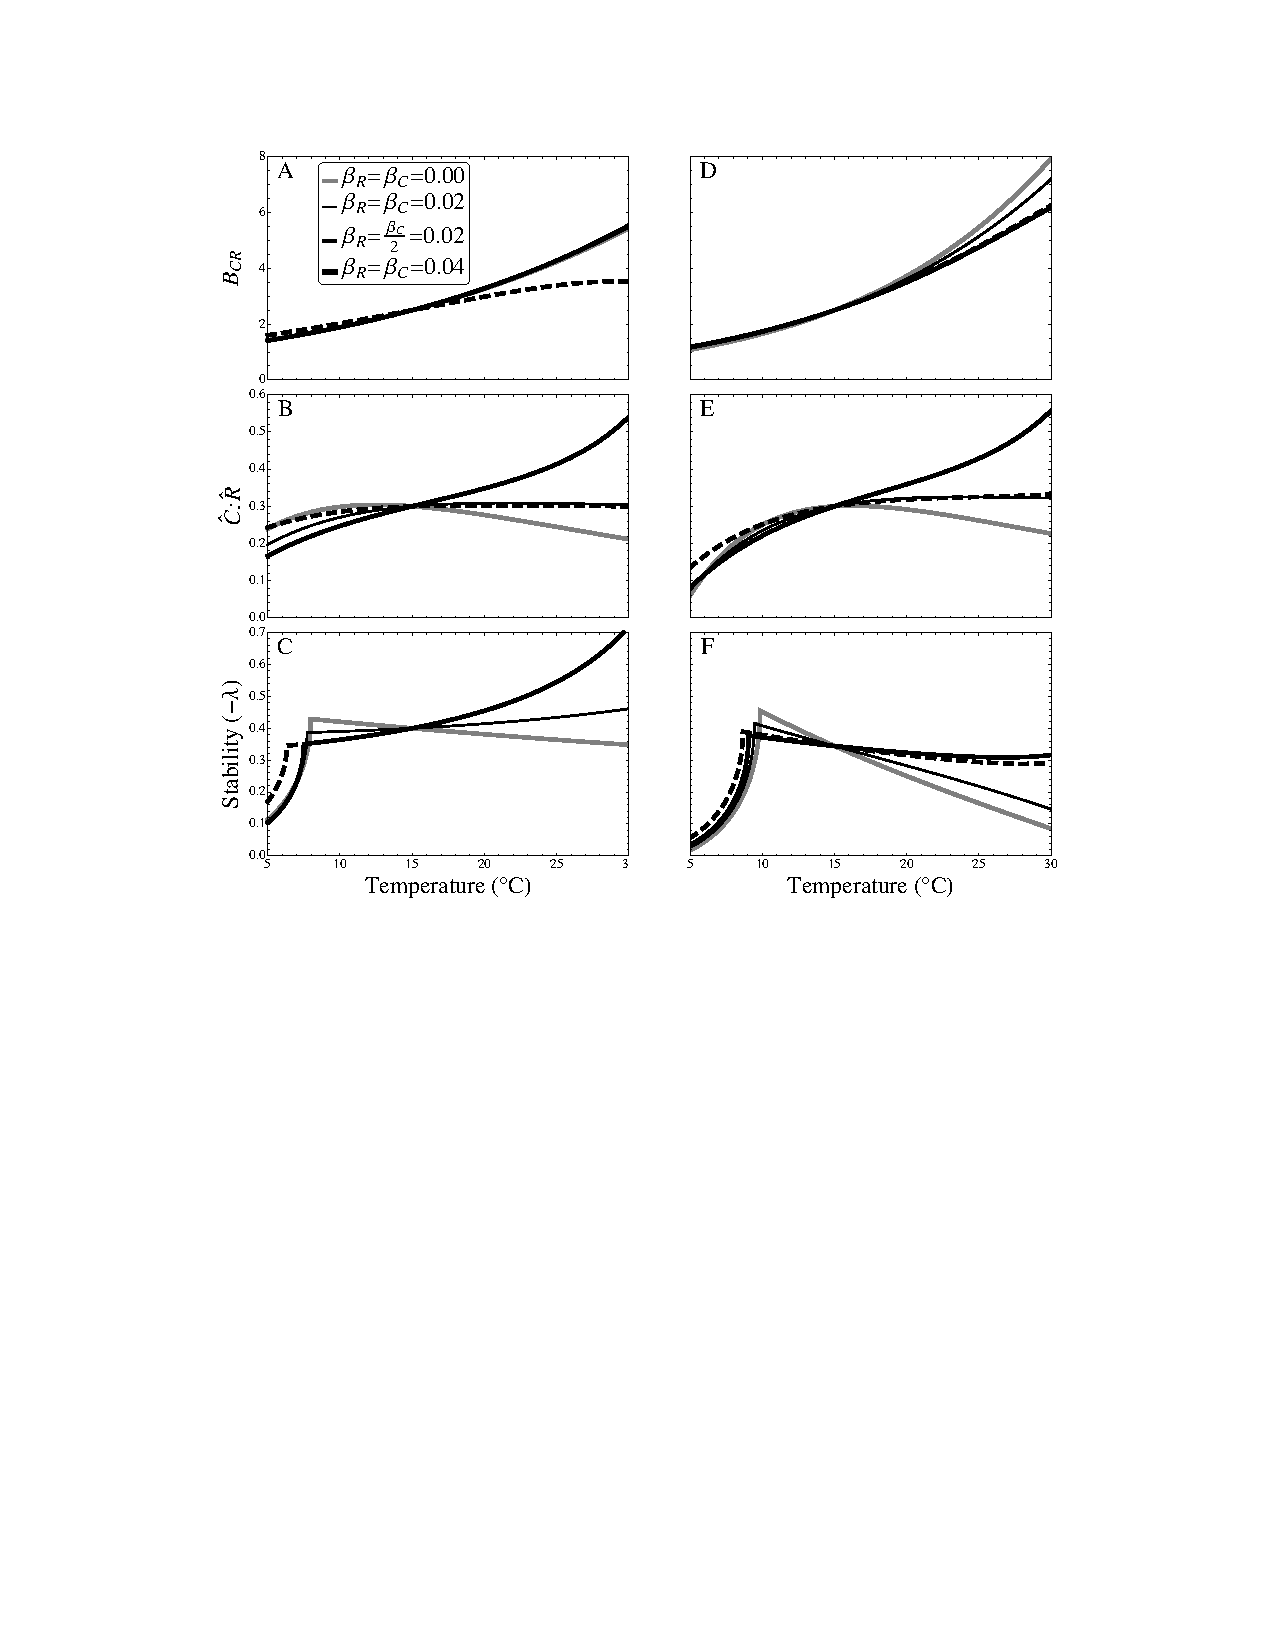
\includegraphics[width=\linewidth, trim = 75 350 75 50, clip]{Figure1.pdf}
\caption{
$B_{CR}$, equilibrium consumer to resource biomass ratio $\hat{C}:\hat{R}$, and stability of the coexistence equilibrium as functions of temperature $T$.
Shown are results with (\textbf{A,B,C}) a type-I functional response and (\textbf{D,E,F}) a type-II functional response, with (\textit{black}) and without (\textit{gray}) the TSR.
Three TSR scenarios are shown: weak symmetric temperature-size responses (\textit{thin, black}), asymmetric temperature-size responses (\textit{dashed, black}), and strong symmetric temperature-size responses (\textit{thick, black}).
Rate-constants ($r_0^*,K_0^*,a_0^*,b_0^*,m_0^*,e_0^*$) were chosen to make $r = 2$, $K = 100$, $f(R) = 0.1$, $m = 0.6$, and $e = 0.15$ at 15$^\circ C$ \citep[as in Figure 3 of][]{Gilbert2014}.
In (\textbf{D,E,F}) we used $h_0^* = 10^{-13}$ such that the coexistence equilibrium was stable over the range of temperatures shown.
Other parameters given in Table \ref{params}.
}
\label{bigfig}
\end{figure}

\newpage
\section*{Table captions}

\begin{table}[!h]
%\begin{tabular}{l l l l}
%\hline
%Parameter & Temperature-dependence & Mass-dependence & Values used \\
%\hline \hline
%$r$ & $ \exp(-E_B / (k T))$ & $M_R^\rho$ & $E_B = 0.32$, $\rho = -0.81$ \\
%$K$ & $ \exp (-(E_S-E_B)/(kT))$ & $M_R^\kappa$ &  $E_S = 0.9$, $\kappa = -0.81$ \\
%$m$ & $ \exp(-E_m/(kT))$ & $M_R^\mu$ & $E_m = 0.65$, $\mu = -0.29$ \\ 
%$a$ & $ (\sum_i [\nu_{0,i} \exp (-E_{\nu,i}/(kT))]^2)^{1/2}$ & $M_C^\alpha$ & $E_{\nu,i} = 0.46$, $\nu_{0,i} = 1$, $\alpha = 1$ \\
%$e$ & none & $M_C^\epsilon$ & $\epsilon = -0.5$\\ 
%$b$ & $ \exp(-E_b/(kT))$ & $M_R^{b_R}M_C^{b_C}$ & $E_b = 0.65$, $b_R = 1/3$, $b_C = 1/4+2/3$\\
%$h$ & $ \exp(-E_h/(kT))$ & $M_R^{h_R}M_C^{h_C}$ & $E_h = -0.65$, $h_R = 0.5$, $h_C = -2/3$ \\
%\hline
%\end{tabular}
\caption{Summary of population dynamic parameters, the form of temperature $T$ and mass $M$ dependency, and the empirical values used to generate the figures. Equations and estimated empirical values come from  \cite{Rall2012}, \citet{Gilbert2014}, and \citet{DeLong2015}; we refer interested readers to these papers for details. Activation energies ($E_i$) have units $eV$ and the Boltzmann's constant is $k = 8.62 \times 10^{-5}$ $eV$/Kelvin.}
\label{params}
\end{table}

%\begin{table}[!h]
%\begin{tabular}{l l l l l}
%\hline
%Parameter & Units & Temperature-dependence & Mass-dependence & Empirical estimates \\
%\hline \hline
%$r$ & time$^{-1}$ biomass$^{-1}$ & $\propto \exp(-E_B / (k T))$ & & $E_B = 0.32$ \\
%$K$ & biomass & $\propto \exp (-(E_S-E_B)/(kT))$ & &  $E_S = 0.9$ \\
%$m$ & time$^{-1}$ biomass$^{-1}$ & $\propto \exp(-E_m/(kT))$ &  & $E_m = 0.65$ \\ 
%$a$ & time$^{-1}$ biomass$^{-2}$ & $\propto (\sum_i [\nu_{0,i} \exp (-E_{\nu,i}/(kT))]^2)^{1/2}$ & &  $E_{\nu,i} = 0.46$, $\nu_{0,i} = 1$ \\
%$e$ & unitless & none (constant) & & \\ 
%$b$ & time$^{-1}$ biomass$^{-2}$ & $\propto \exp(-E_b/(kT))$ & & $E_b = 0.65$\\
%$h$ & time biomass? & $\propto \exp(-E_h/(kT))$ & & $E_h = -0.65$ \\
%\hline
%\end{tabular}
%\end{table}

\end{document}
